%%%%%%%%%%%%%%%%%%%%%%%%%%%%%%%%%%%%%%%%%
% University/School Laboratory Report
% LaTeX Template
% Version 3.1 (25/3/14)
%
% This template has been downloaded from:
% http://www.LaTeXTemplates.com
%
% Original author:
% Linux and Unix Users Group at Virginia Tech Wiki 
% (https://vtluug.org/wiki/Example_LaTeX_chem_lab_report)
%
% License:
% CC BY-NC-SA 3.0 (http://creativecommons.org/licenses/by-nc-sa/3.0/)
%
%%%%%%%%%%%%%%%%%%%%%%%%%%%%%%%%%%%%%%%%%

%----------------------------------------------------------------------------------------
%	PACKAGES AND DOCUMENT CONFIGURATIONS
%----------------------------------------------------------------------------------------

\documentclass{article}

\usepackage{graphicx} % Required for the inclusion of images
\usepackage{natbib} % Required to change bibliography style to APA
\usepackage{amsmath} % Required for some math elements 
\usepackage{amsthm}
\usepackage[hyphens]{url}
\usepackage{hyperref}
\usepackage{subcaption}
\usepackage{float}
\usepackage{array}
\usepackage{amssymb}
\usepackage{calrsfs}
\usepackage{pgfplots}
\pgfplotsset{width=10cm,compat=1.9}
\usepackage{bytefield}


\setlength\parindent{0pt} % Removes all indentation from paragraphs

\newtheorem*{remark}{Theorem}
\newtheorem*{definition}{Definition}

%----------------------------------------------------------------------------------------
%	DOCUMENT INFORMATION
%----------------------------------------------------------------------------------------

\title{Homework \#5 \\Telegram vs WhatsApp Security \\[0.2em]\small{}CNS Course Sapienza} % Title and subtitle

\author{Riccardo \textsc{Prinzivalle}, 1904064} % Author name

\date{November 30, 2020} % Date for the report

\begin{document}

\maketitle % Insert the title, author and date

%----------------------------------------------------------------------------------------
%	SECTION 0
%----------------------------------------------------------------------------------------

\section{Homework Goal}

This homework contains a comparison of Telegram and WhatsApp security, with an in deep to protocols comparisons and past and some current threat an vulnerabilities.

%----------------------------------------------------------------------------------------
%	SECTION 1
%----------------------------------------------------------------------------------------

\section{Telegram Security basics}

Telegram uses a security protocol called MTProto, developed by the telegram team. It is a symmetric encryption protocol based on 256-bit symmetric AES encryption, 2048-bit RSA encryption and Diffie–Hellman key exchange. The protocol is divided in 3 layers:

\begin{itemize}
	\item \textbf{High-level} component which defines the method whereby API queries and responses are converted to binary messages.
	\item  \textbf{Cryptographic/authorization} layer which defines the method used to encrypt messages prior to being transmitted through the transport protocol.
	\item  \textbf{Transport} component, which defines the method for the client and the server to transmit messages over some other existing network protocol.
\end{itemize}

Let's analyze in the details every section. The high level component sees a client and a server exchanging messages inside a session, which is identified by a user key identifier (a particularity, the session is attached to the client instead of standard protocols such as http/s or tcp). The client can instantiate different connections to the server (the practicality of Telegram stands in the fact that one can open different sessions on many devices such as browsers without having to log in many times once one have the session active), and messages can be sent from one connection to the other and everything is synchronized server side. The low level message structure can be seen in fig. \ref{fig:tel_pack}.

\begin{figure}[H]
	\centering
	\begin{bytefield}[bitwidth=0.55em]{64}
		\bitheader{0,4,8,12,16,20,24,28,32,36,40,44,48,52,56,60,64} \\
		\begin{rightwordgroup}{encryption \\ header}
			\bitbox{64}{key identifier} \\
			\wordbox[tlr]{1}{message key} \\
			\wordbox[blr]{1}{128 bit} \\
		\end{rightwordgroup} \\
		\begin{rightwordgroup}{message \\ body}
			\bitbox{64}{message identifier} \\
			\bitbox{32}{message sequence number} & \bitbox{32}{message length} \\
			\wordbox[tlr]{3}{message body (32 bit multiple)} \\
			\bitbox[blr]{32}{}
			& \bitbox{32}{type dependent parameters}
		\end{rightwordgroup} \\
	\end{bytefield}
	\caption{Telegram simplified packet structure}
	\label{fig:tel_pack}
\end{figure}

To be mentioned, all number are saved as little endian, with the exception of large numbers, such as those needed by RSA and DH which are stored as big endian due to openSSL compatibility.\newline
The encryption part can be identified in the upper part fig. \ref{fig:tel_pack}: the message is encrypted using a 256-bit key constituted by the message key and the user key and the encryption is performed with AES-256. The message key is defined as the hash using SHA256 on the message body, and taking the 128 middle resulting bits. The user key is generated from the authorization key: it is created once, when the client is first run on the device, and never changes, so this will expose all messages if that key is stolen (even from the device or from server side); different counter measures can be taken: 

\begin{itemize}
	\item Use session keys generated at every session using the Diffie Hellman exchange protocol
	\item Store the keys on the device and protect them with a password
	\item Protect all stored and cached data of the device with a password
\end{itemize}

All these measures cannot protect the user in the case where is the server that is violated or some government agency ask the keys for terrorism prevention (as example). The complete encryption scheme for every message can be seen in fig \ref{fig:Tel_enc}.

\begin{figure}[H]
	\centering
	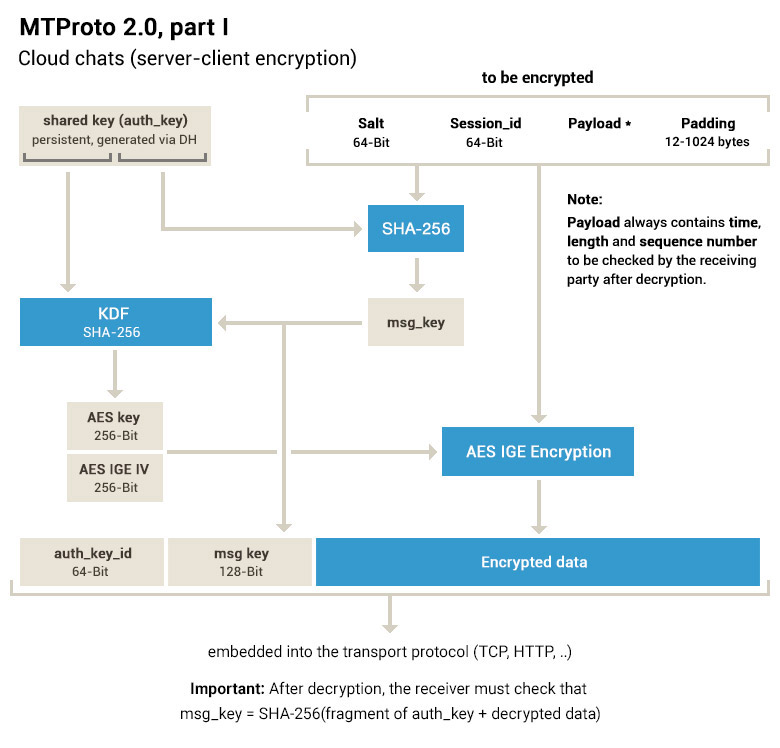
\includegraphics[width=0.9\textwidth]{images/mt_p1.jpg}
	\caption{MTProto}
	\label{fig:MTProto}
\end{figure}


\begin{figure}[H]
	\centering
	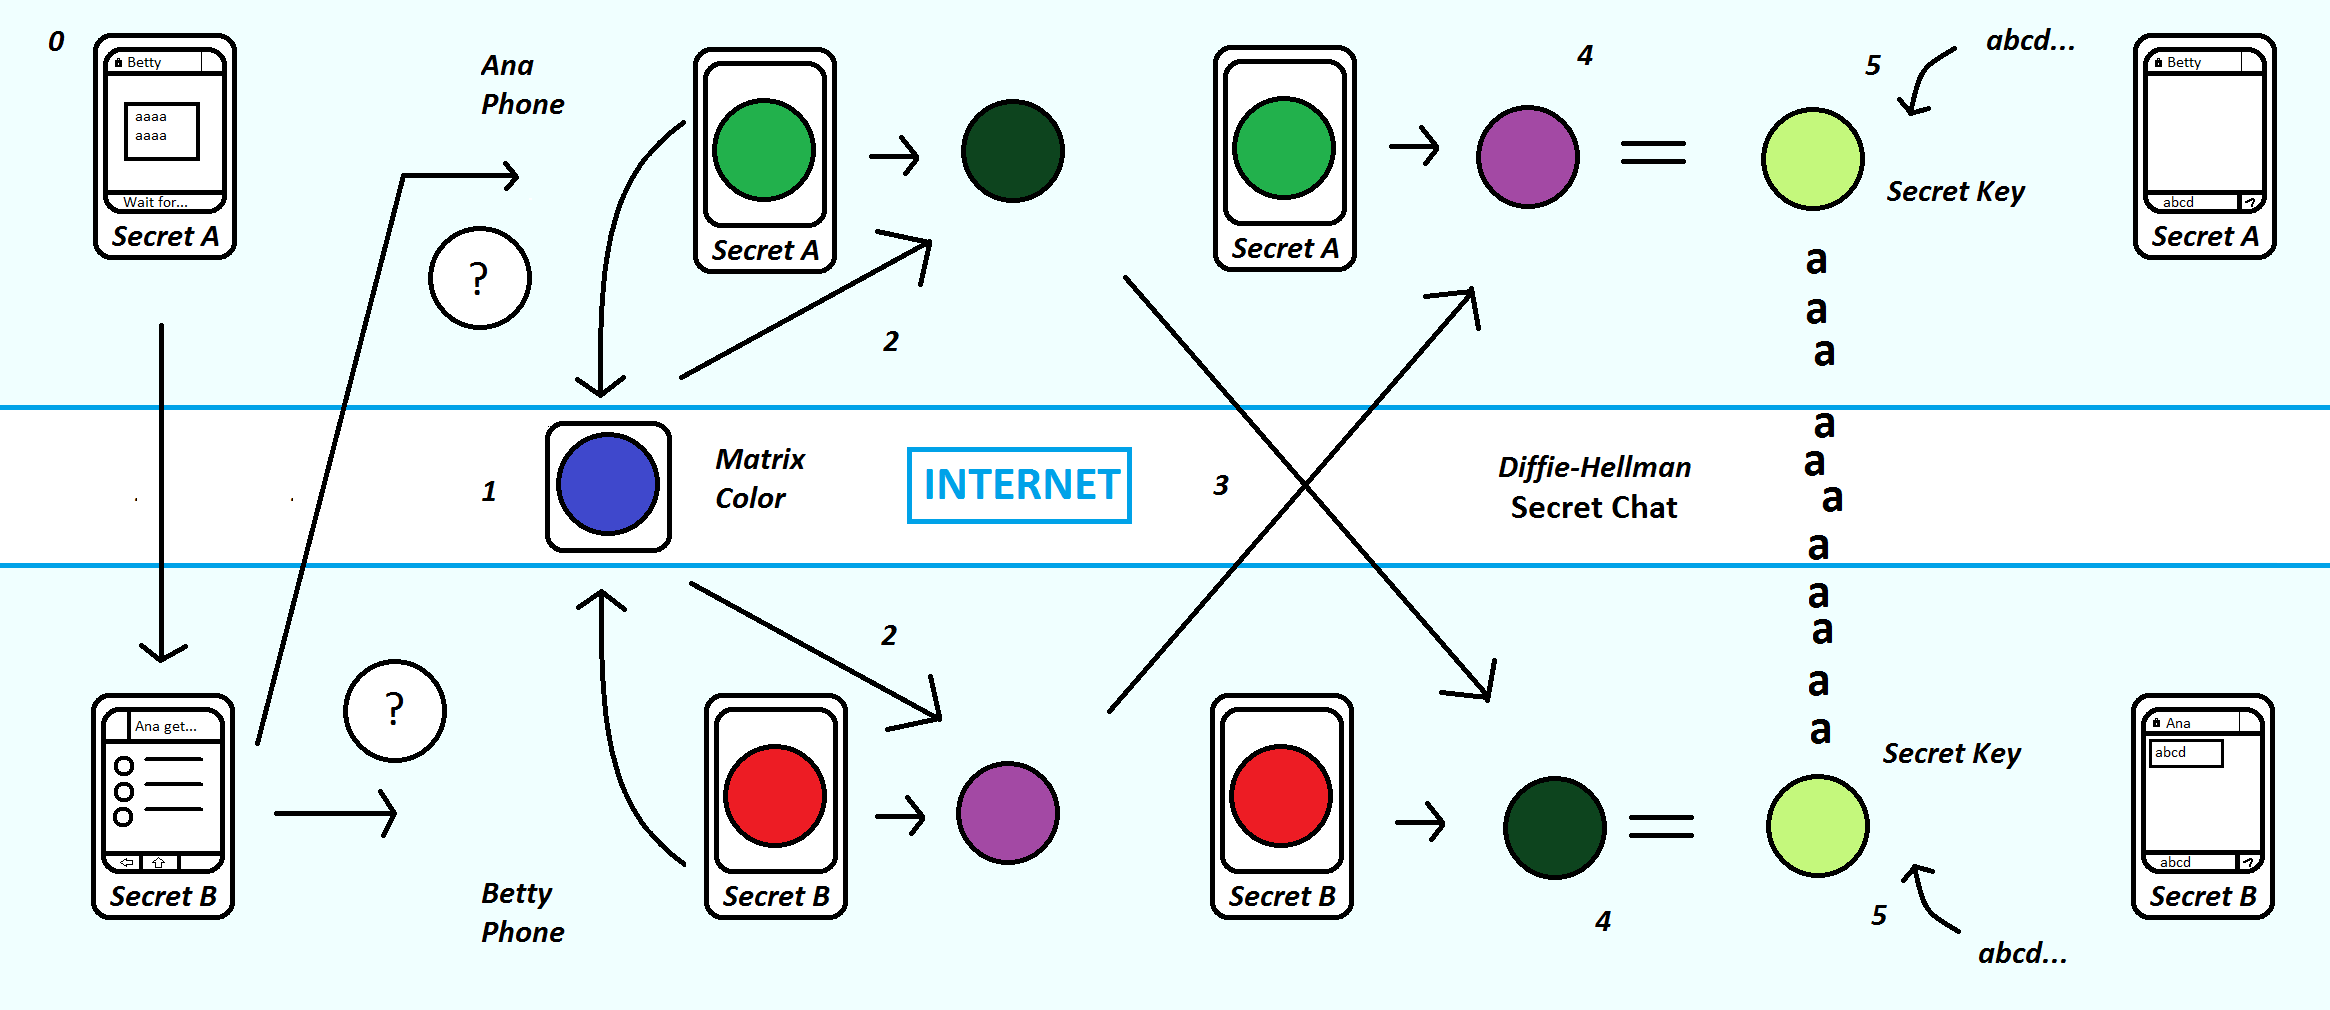
\includegraphics[width=0.9\textwidth]{images/Explanation_of_secret_chats_(Telegram)}
	\caption{Telegram encryption scheme \cite{tel_scheme}}
	\label{fig:Tel_enc}
\end{figure}

%----------------------------------------------------------------------------------------
%	SECTION 3
%----------------------------------------------------------------------------------------

\section{WhatsApp Security Basics}



%----------------------------------------------------------------------------------------
%	SECTION 4
%----------------------------------------------------------------------------------------

\section{Protocols comparison}


 
%----------------------------------------------------------------------------------------
%	SECTION 5
%----------------------------------------------------------------------------------------

\section{Past Evolution and Fixed Vulnerabilities}



%----------------------------------------------------------------------------------------
%	SECTION 6
%----------------------------------------------------------------------------------------

\section{Current Vulnerabilities and Security Threats}

%----------------------------------------------------------------------------------------
%	SECTION 7
%----------------------------------------------------------------------------------------

\section{Conclusion}

After this brief introduction on elliptic curves, it is obvious why they have been widely adopted in many cases of asymmetric encryption: they use less bits for the same level of security, so are more efficient to compute and their base concepts are easier to visualize. As suggested on section , EC can be easily used in hybrid encryption scheme, in the key exchange phase.

%----------------------------------------------------------------------------------------
%	BIBLIOGRAPHY
%----------------------------------------------------------------------------------------

\bibliographystyle{abbrv}

\bibliography{biblio}

%----------------------------------------------------------------------------------------


\end{document}